% --- Bayesan Networks ---
\begin{tikzpicture}
    \node [mybox] (box)
    {%
        \begin{minipage}{0.48\textwidth}
        \begin{tabular}{lp{0.48\textwidth} l}
            % --- Bayesan Networks ---
            Bayesan Network:
            &
            a DAG where Nodes represent random variables and edges represent direct influence.

            \begin{tikzpicture}
                \node (X_1) at (0,0) {Cloudy};
                \node (X_2) at (-1.5,-1.5) {Sprinkler};
                \node (X_3) at (1.5,-1.5) {Rain};
                \node (X_4) at (0,-3) {WetGrass};

            \draw[->](X_1)--(X_2);
            \draw[->](X_1)--(X_3);
            \draw[->](X_2)--(X_4);
            \draw[->](X_3)--(X_4);
            \end{tikzpicture}
            \\

            % -- Conditional Independence ---
            Conditional Independence:
            &
            $P(X_1 | X_2, X_3) = P(X_1 | X_3)$

            then $X_1$ and $X_2$ are conditionally independent given $X_3$

            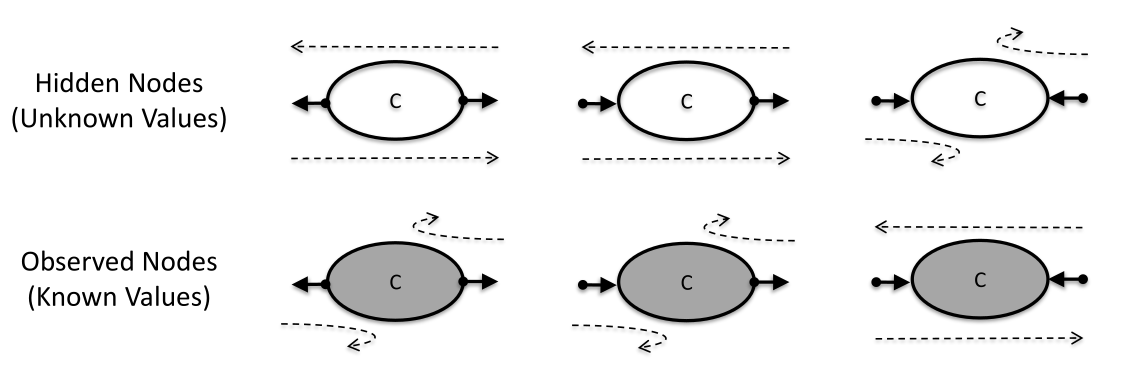
\includegraphics[width=0.48\textwidth]{imgs/01_conditional_indipendence.png}
            
            Two (sets of) nodes $A$ and $B$ are conditionally independent (d-separated) given $C$ if and only if all the path from $A$ to $B$ are shielded by $C$.

            \\

            % --- Joint Distribution Factorization ---
            Joint Distribution Factorization:
            &
            $P(X_1,\ldots, X_n) = \prod_{i=1}^{n} P(X_i | \text{pa}(X_i))$

            \\

            % --- Explaining Away ---
            Explaining Away:
            &
            describes two variable which become dependent because you observe a third one.
        \end{tabular}

        \end{minipage}
    };

%------------ Bayesan Networks Header ---------------------
\node[fancytitle, right=10pt] at (box.north west) {Bayesan Networks};
\end{tikzpicture}